\begin{frame}{Explanations}
	Here we focus on \alert{explainability}, characterized by
	\vspace{1em}

	\begin{quote}
		An active characteristic of a model, denoting any action or procedure taken by a model with the intent of clarifying or detailing its internal functions~\cite{Arrieta2019}.
	\end{quote}

	We consider \alert{attribution} techniques and \alert{counterfactual} explanations. 

\end{frame}

\begin{frame}{Attribution Techniques}
	\begin{itemize}
		\item Identifies contribution of each input feature wrt. the output
		\item ``Gradient-like'' computations
		\item Based on different propagation rules
	\end{itemize}
	
	\begin{figure}
		\centering
		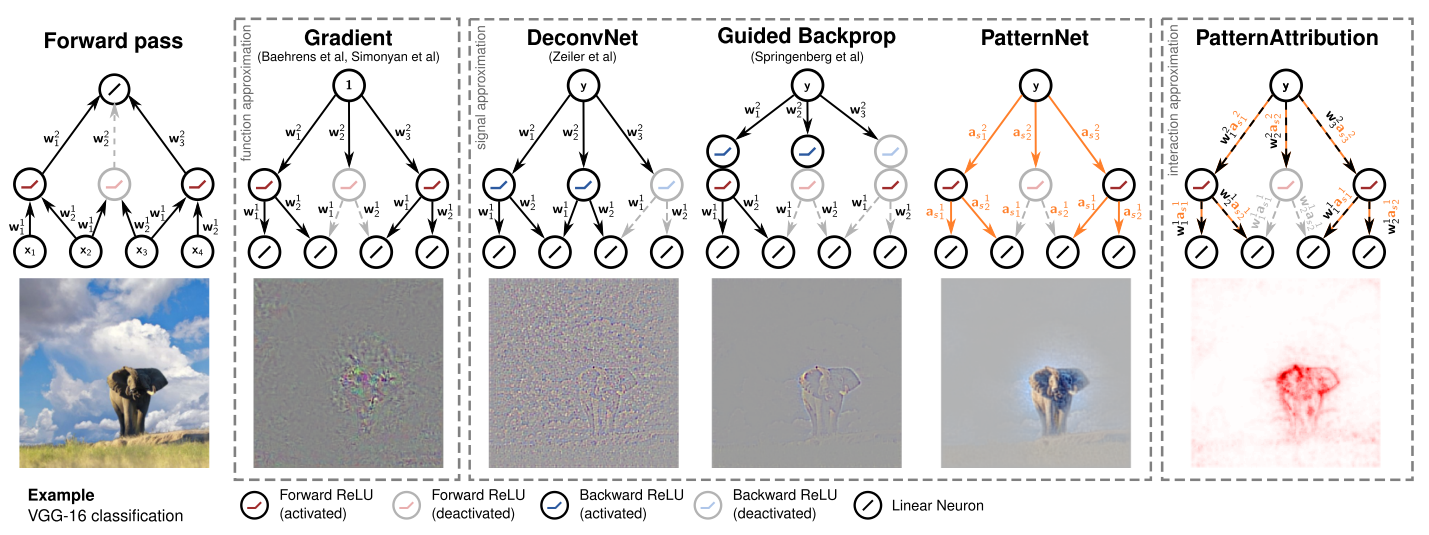
\includegraphics[width=0.8\textwidth]{explanation_techniques}
		\caption{Direct copy from~\cite{patternnet}.}
	\end{figure}
\end{frame}

\begin{frame}{Counterfactual Explanations}

	Counterfactual explanations tries to answer the question 
	\vspace{1em}

	\begin{quote}
		How can I make a \alert{minimal} and \alert{realistic} change to an input of the model such that the predicted outcome changes?
	\end{quote}
	\vspace{1em}

	\begin{columns}
		\begin{column}{0.5\textwidth}
			\alert{Common strategy}
			\begin{enumerate}
				\item Start from the original input
				\item Until prediction change
					\begin{enumerate}
						\item Make small change to the input
						\item Query the classifier to gain information
					\end{enumerate}
			\end{enumerate}
		\end{column}
		\begin{column}{0.5\textwidth}
			\alert{Differences}
			\begin{itemize}
				\item How to do update
				\item Information gained from classifier
			\end{itemize}
		\end{column}
	\end{columns}

\end{frame}

\begin{frame}[standout]
	Improving Explanations with Probabilistic Saliency Estimation
\end{frame}

\begin{frame}{Probabilistic Saliency Estimation}

\end{frame}

\begin{frame}{Area Under Perturbation Score}

\end{frame}

\begin{frame}[standout]
	Attention Mechanisms in Gradient Explanations
\end{frame}

\begin{frame}{Explanations Relies on Gradients}
	% Generalization
	% Guided Back Prop as example
\end{frame} 





\begin{frame}{Issues}
	% Loss for attribution functions?
\end{frame}

\begin{frame}[standout]
	Generating Counterfactual Explanations
\end{frame}


\begin{frame}{Construction}
	$$
	f(x) = \sigma \left ( \beta^T NN(x) \right)
	$$

	$$
	f^\dagger(y) = NN^{-1}\left( f(x) - \frac{f(x)^T \beta}{||\beta||}\right)
	$$
\end{frame}

